\section{Cryptographic wallets}
\label{sec:blockchain-wallets}
\providecommand{\WalletOverviewFigure}{
	\begin{figure}[htbp]
		\centering
		\begin{tikzpicture}[
			node distance=1.2cm and 1.6cm,
			every node/.style={font=\footnotesize\ttfamily},
			align=center,
			box/.style={draw, minimum width=4.2cm, minimum height=3.6cm}
			]
			
			\node[box] (wallet1) {
				Wallet 1\\[0.3cm]
				Secret key:\\
				0245a349...6130\\[0.3cm]
				Public key:\\
				0357048e...ce2b
			};
			
			\node[box, right=of wallet1] (wallet2) {
				Wallet 2\\[0.3cm]
				Secret key:\\
				df60ed2d...f9bb\\[0.3cm]
				Public key X:\\
				d50cf8d1...ed45\\[0.3cm]
				Public key Y:\\
				71bf8c8b...e08e
			};
			
			\node[box, right=of wallet2] (wallet3) {
				Wallet 3\\[0.3cm]
				Secret key:\\
				8c10c0c2...42e6\\[0.3cm]
				Public key:\\
				037f9449...a3abc
			};
			
			\node[below=2.6cm of wallet1] (addr1) {\shortstack{Address (BTC)\\16tay2XDBFSV3tBpTNfHCyRAt\\WarT1hWdE}};
			\node[below=2.6cm of wallet2] (addr2) {\shortstack{Address (ETH)\\0x35a53747aba81a63\\579b6c534d16db98\\1d677889}};
			\node[below=2.6cm of wallet3] (addr3) {\shortstack{Address (BTC)\\18kh6FQB7QwC9NBynN7pNWhe\\b6CmsDNSdR}};
			
			\draw[->] (wallet1.south) -- node[right, yshift=-4pt] {\scriptsize Derivation} (addr1.north);
			\draw[->] (wallet2.south) -- node[right, yshift=-4pt] {\scriptsize Derivation} (addr2.north);
			\draw[->] (wallet3.south) -- node[right, yshift=-4pt] {\scriptsize Derivation} (addr3.north);
			
			\node[fit=(wallet1)(wallet2), draw, dashed, label=above:{Account 1}, inner sep=0.5cm, minimum height=5.1cm] (acc1) {};
			\node[fit=(wallet3), draw, dashed, label=above:{Account 2}, inner sep=0.5cm, minimum height=5.1cm] (acc2) {};
			
			\node[fit=(acc1)(acc2), draw, dashed, label=above:{Example identity}, inner sep=0.5cm] (identity) {};
			
		\end{tikzpicture}
		\caption{Relationship between identity, accounts, wallets, key pairs, and blockchain addresses.}
		\label{fig:wallet-overview}
	\end{figure}
}

\providecommand{\BIPWalletFigure}{
	\begin{figure}[htbp]
		\centering
		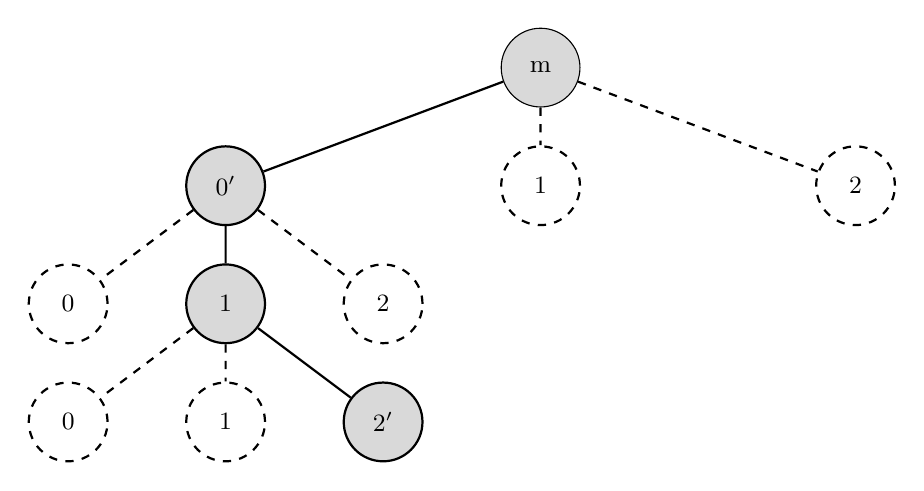
\begin{tikzpicture}[
			level 1/.style={sibling distance=4cm},
			level 2/.style={sibling distance=2cm},
			level 3/.style={sibling distance=2cm},
			every node/.style={circle, draw, minimum size=1cm, align=center, font=\small},
			selected/.style={fill=gray!30},
			dashed edge/.style={draw, thick, dashed},
			solid edge/.style={draw, thick}
			]
			
			\node[selected]{m}
			child[solid edge] {node[selected] {$0'$}
				child[dashed edge] {node {0}}
				child[solid edge] {node[selected] {1}
					child[dashed edge] {node {0}}
					child[dashed edge] {node {1}}
					child[solid edge] {node[selected] {$2'$}}
				}
				child[dashed edge] {node {2}}
			}
			child[dashed edge] {node {1}}
			child[dashed edge] {node {2}};
			
		\end{tikzpicture}
		\caption{Derivation path $m/0'/1/2'$ in a BIP32 hierarchical tree.}
		\label{fig:bip32-path}
	\end{figure}
}

\providecommand{\StatefulWalletFigure}{	
	\begin{figure}[htbp]
		\centering
		\begin{tikzpicture}[
			every node/.style={font=\sffamily\small},
			box/.style={draw, fill=gray!20, rounded corners, minimum width=1.4cm, minimum height=0.9cm, align=center},
			proc/.style={draw, rounded corners, minimum width=1.6cm, minimum height=0.9cm},
			arrow/.style={-Stealth, thick},
			]
			
			\node[proc] (keygen) at (0,0) {\texttt{KeyGen}};
			
			\node[box] (pk0) at (2.2,1.8) {pk\textsubscript{0}};
			\node[box] (sk0) at (2.2,-1.8) {sk\textsubscript{0}};
			\node[box] (st) at ($(pk0)!0.5!(sk0)$) {$st$}; % <-- Neu positioniert in der Mitte
			
			\node[box] (id) at (4.5,0) {$i$};
			
			\node[proc] (pkder) at (4.5,1.8) {\texttt{PKDer}};
			\node[proc] (skder) at (4.5,-1.8) {\texttt{SKDer}};
			
			\node[box] (pki) at (6.7,1.8) {pk\textsubscript{i}};
			\node[box] (ski) at (6.7,-1.8) {sk\textsubscript{i}};
			
			\draw[arrow] (keygen) -- (st);
			\draw[arrow] (st) -- (pk0);
			\draw[arrow] (st) -- (sk0);
			
			\draw[arrow] (pk0) -- (pkder);
			\draw[arrow] (st) -- (pkder);
			\draw[arrow] (id) -- (pkder);
			\draw[arrow] (pkder) -- (pki);
			
			\draw[arrow] (sk0) -- (skder);
			\draw[arrow] (st) -- (skder);
			\draw[arrow] (id) -- (skder);
			\draw[arrow] (skder) -- (ski);
			
		\end{tikzpicture}
		\caption{Session key derivation in a stateful wallet}
		\label{fig:stateful-wallet}
	\end{figure}
}


\paragraph{Definition and purpose}
A cryptographic wallet is a data structure that manages pairs of secret and public keys. These keys are used to authorize blockchain transactions and to demonstrate control over specific addresses. Ownership of assets is not determined by the wallet itself but by the ability to generate valid digital signatures with the corresponding secret key. In most blockchain protocols, addresses are derived from public keys via cryptographic hash functions (e.g., RIPEMD-160 in Bitcoin or Keccak-256 in Ethereum)~\cite{buterin2014ethereum}. Public keys therefore constitute the cryptographic basis from which blockchain-specific addresses are generated. Since this work does not rely on address semantics, wallets are represented directly by their public keys, independent of protocol-specific address formats. Beyond transaction authorization, recent work has highlighted the emerging role of wallets as cryptographic anchors in decentralized identity systems, where they enable secure key derivation and verifiable user control~\cite{Das2019,Das2021}.


\paragraph{Wallet types}
From a key management perspective, wallets can be classified into non-deterministic, deterministic, and hierarchical deterministic (HD) designs \cite{antonopoulos2023}. Non-deterministic wallets generate each key independently using fresh randomness, offering high entropy and forward secrecy, but suffering from backup complexity and lack of structure \cite{narayanan2016bitcoin}. Deterministic wallets resolve this by using a fixed root secret (the master seed) from which all subsequent key pairs are derived using deterministic key derivation functions \cite{Das2019}. HD wallets, a subclass of deterministic wallets, extend this idea by introducing a tree structure that enables organized derivation of keys for different applications, accounts, or assets \cite{bip32, bip44}. This model supports structured backups, flexible key derivation, and organized key separation across applications or accounts \cite{antonopoulos2023}.

\paragraph{\acrshort{hd} wallets}
The \acrshort{hd} wallet standard is specified across the three key Bitcoin Improvement Proposals \acrshort{bip32}, \acrshort{bip39}, and \acrshort{bip44}~\cite{bip32,bip39,bip44}. In addition, \acrshort{hd} wallets are widely used in modern decentralized systems and are implemented in software, hardware, and browser-based environments. The core functionality of these wallets is formalized below. Although there is no formal cryptographic definition of \acrshort{hd} wallets in the literature, the following description summarizes their core functions as implemented in \acrshort{bip32}-based schemes.

\begin{definition}[\acrshort{hd} Wallet]
	A \textit{\acrshort{hd} wallet} is a deterministic key management scheme specified by the following algorithms:
	
	\begin{itemize}
		\item $(pk_0, sk_0, cc_0) \leftarrow \texttt{KeyGen}(s)$: A \acrfull{ppt} algorithm that takes as input a uniformly random seed $s$ and outputs a master secret key $sk_0$, a corresponding public key $pk_0$, and a chain code $cc_0$.
		
		\item $(sk_i \text{ or } pk_i, cc_i) \leftarrow \texttt{KeyDer}(sk_p, pk_p, cc_p, i)$: A deterministic algorithm that takes as input a parent key pair $(sk_p, pk_p)$, a chain code $cc_p$, and an index $i$, and outputs a child key $sk_i$ or $pk_i$ and a new chain code $cc_i$.\footnote{The \texttt{KeyDer} function abstracts over both hardened and non-hardened derivations as defined in the \acrshort{bip32} specification. The exact derivation logic is shown in Table~\ref{tab:hd-derivation}.}
		
		\item $\sigma \leftarrow \texttt{Sign}(sk, m)$: A deterministic signing algorithm that takes as input a secret key $sk$ and a message $m$, and outputs a digital signature $\sigma$ over $m$.
		
		\item $b \leftarrow \texttt{Verify}(pk, m, \sigma)$: A deterministic verification algorithm that takes as input a public key $pk$, a message $m$, and a signature $\sigma$, and outputs a bit $b \in \{0,1\}$, where $b = 1$ if $\sigma$ is a valid signature on $m$ under $pk$, and $b = 0$ otherwise.
	\end{itemize}
\end{definition}

These functions form the foundation for secure key management, identity binding, and transaction authorization in blockchain applications. Furthermore, \acrshort{bip32} defines how keys and associated chain codes are recursively derived in a tree structure. Each node can produce child keys either through non-hardened or hardened derivation paths. Non-hardened derivations allow public key delegation, where child public keys can be derived from a parent public key and chain code. Hardened derivations require the parent secret key and prevent certain compromise scenarios like recovering a parent secret key from a child secret key and the parent public key. The derivation process begins with a root seed, which is converted into a master key and chain code as defined above by the \texttt{KeyGen} algorithm. Subsequent child keys are derived recursively using the algorithms specified in table~\ref{tab:hd-derivation}.

\begin{table}[htbp]
	\centering
	\begin{tabular}{c|c}
		\toprule
		\textbf{Non-hardened derivation} & \textbf{Hardened derivation} \\
		\midrule
		Secret key derivation: & Secret key derivation: \\
		$(sk_i, cc_i) \leftarrow \texttt{KeyDer}(sk_p, cc_p, i)$ & $(sk_i, cc_i) \leftarrow \texttt{KeyDer}(sk_p, cc_p, i')$ \\
		Public key derivation: & Public key derivation: \\
		$(pk_i, cc_i) \leftarrow \texttt{KeyDer}(pk_p, cc_p, i)$ & $pk_i \leftarrow \texttt{KeyDer}(sk_i)$ \\
		\bottomrule
	\end{tabular}
	\caption{Comparison of \acrshort{bip32} derivation types.}
	\label{tab:hd-derivation}
\end{table}

In most blockchain applications, \acrshort{hd} wallets are instantiated over elliptic-curve key pairs based on \acrshort{ecdsa} with the curve \emph{secp256k1}. This curve is specified by the Standards for Efficient Cryptography Group (SECG) and widely used in Bitcoin and Ethereum~\cite{SEC2}. It is also listed among the cryptographic algorithms approved for use in the EU context~\cite{SOGIS-ACM-1.3}.

Each key in the \acrshort{hd} wallet hierarchy is identified using a path notation of the form \texttt{m/level1/level2/.}. Hardened derivations are denoted by an apostrophe, e.g., \texttt{m/44'/0'/0'/0/0}. \acrshort{bip39} introduces mnemonic phrases as a human-readable representation of the master seed, improving usability and security. \acrshort{bip44} further formalizes the derivation path into five semantic levels: \texttt{m / purpose' / coin\_type' / account' / change / address\_index}. This allows wallet applications to organize keys for different cryptocurrencies, user accounts, and address purposes in a standardized and interoperable way. For the purposes of this thesis, we abstract from the full \acrshort{bip44} hierarchy and adopt a flat derivation model. Concretely, the designated parent key $pk_0$ is placed at the account level (\texttt{m/44'/0'/0'}), and child keys $pk_i$ are derived in a single non-hardened step as \texttt{m/44'/0'/0'/i}, thereby omitting the intermediate \texttt{change} and \texttt{address\_index} levels. Figure~\ref{fig:bip32-path} illustrates a derivation path within the \acrshort{bip32} hierarchical tree.

\BIPWalletFigure

\paragraph{Stateful wallets}
This type of wallet extends deterministic key derivation by introducing an internal state that evolves over time. \acrshort{hd} wallets as defined in \acrshort{bip32}~\cite{bip32} are stateless. Every key can be recomputed solely from the seed and index, and no information about past derivations is stored. In contrast, stateful wallets maintain an additional parameter \emph{st} that is updated on each derivation, for example by incrementing a counter or recording previously used indices. This evolving state enables advanced key management patterns such as controlled key rotation, one-time keys, or unlinkable session identifiers. Even if the same index is reused, the derivation yields different results, supporting properties like forward secrecy and prevention of address reuse. Structurally, stateful wallets still rely on a seed-based hierarchy but deviate from the fixed tree structure of \acrshort{hd} wallets. As a result, some interoperability guarantees of \acrshort{bip32}-compliant designs are lost, while more dynamic and context-sensitive key derivation strategies become possible, which are particularly relevant in identity-oriented systems~\cite{Das2021,erinle2025sokdesignvulnerabilitiessecurity}.
